\documentclass[11pt, a4paper]{article}
\usepackage{graphicx}
\usepackage{amsmath}
\usepackage[margin=0.6in]{geometry}
\usepackage{listings}
\usepackage{float}

\title{EE2703: Assignment 3}
\author{Sagar (ee20b115)}
\date{\today} 

\begin{document}
    \maketitle 

    \section{AIM}
        In this assignment we aim to :
        \begin{itemize}
            \item Observe the error in fitting the Least Error Fit function to a given set of data.
            \item Find the relation between the error observed and the noise in the data.
        \end{itemize}
   
    \section{PROCEDURE}
        The function to be fitted is:
        \begin{equation}
            f(t) = 1.05J_2(t)-0.105t
        \end{equation}
        where $J_2(t)$ is the 'Bessel Function of the first kind  and of Order 2'. The true data is obtained using this equation.

        \subsection{Creating data with random noise}
            To create data with random noise, we add random noise to $f(t)$. This random noise, denoted by $n(t)$, is given by the standard normal probability distribution:
            \begin{equation}
                P(n(t)|\sigma)=\frac{1}{\sqrt{2\pi\sigma^2}}e^{-\frac{n(t)^2}{2\sigma^2}} \label{eq1}
            \end{equation}
            The resulting data will be of the form:
            \begin{equation}
                f(t) = 1.05J_2(t)-0.105t+n_{\sigma_i}(t)
            \end{equation}
            where, $n_{\sigma_i}(t)$ is the noisy data function with $\sigma = \sigma_{i}$ in \eqref{eq1}. Thus for 9 values of $\sigma$, the noisy data is created and stored in 'fitting.dat' file.

        \subsection{Analyzing the data with noise included}
            The output result looks as follows:
            \begin{figure}[H]
                \centering
                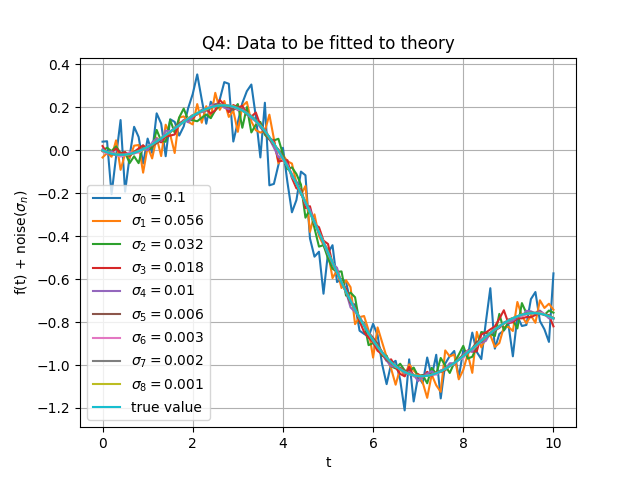
\includegraphics[scale=0.5]{figure_0.png}
                \caption{Noisy Data with True Data}
                \label{fig:figure_0}
            \end{figure}

            As can be observed, the inaccuracy of the data increases with increasing $\sigma$. We can also observe this using 'errorbar' plot in python:
            \begin{figure}[H]
                \centering
                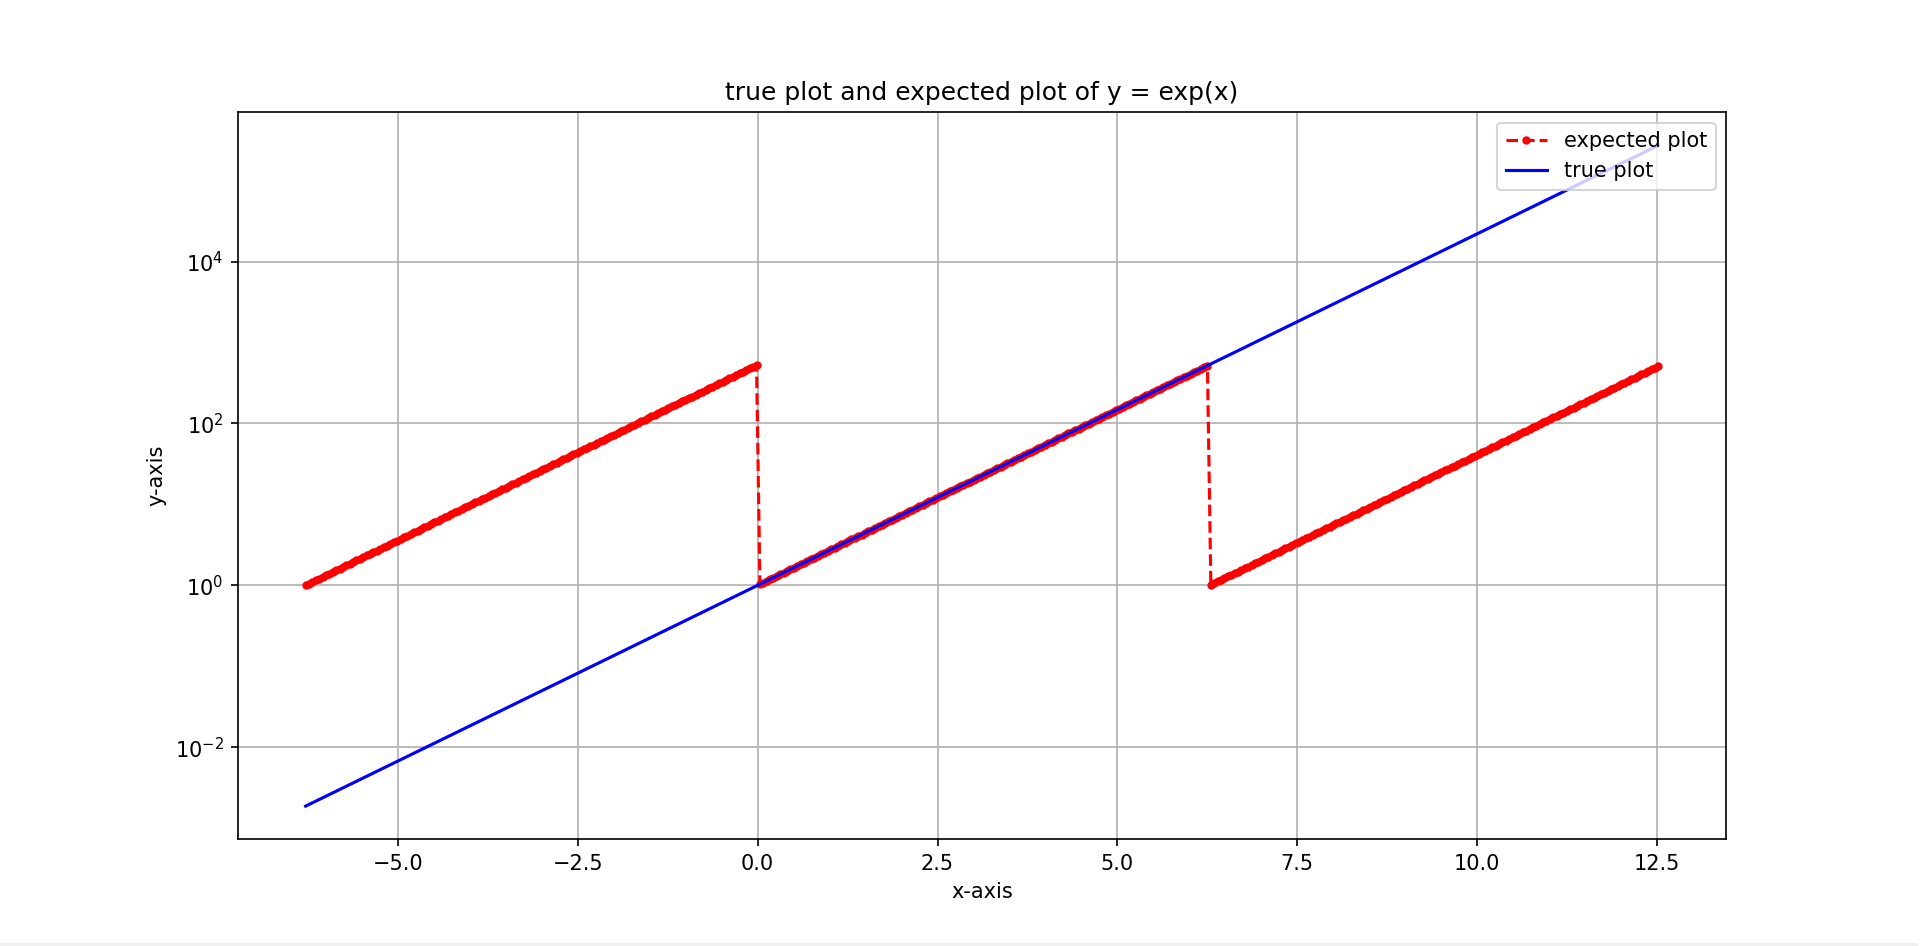
\includegraphics[scale=0.5]{figure_1.png}
                \caption{Noisy Data with Errorbar}
                \label{fig:figure_1}
            \end{figure}

            The cyan lines (error bar) indicate the standard deviation of the noisy data from the original data. It is plotted for every $5^\text{th}$ point.

        \subsection{Finding an approximation for data with noise included}
            From the data, we can conclude that the data can be fitted into a function of the form:
            \begin{equation}
                g(t, A, B) = AJ_2(t)+Bt
            \end{equation}
            where $A$ and $B$ are constants that we need to find.\\

            To find the coefficients $A$ and $B$, we first try to find the mean square error between the function and the data for a range of values of \textit{A} and \textit{B}, which is given by:
            \begin{equation}
                \epsilon_{ij} = \frac{1}{101}\sum_{k=0}^{101}(f(t_k) - g(t_k, A_i, B_j))^2
            \end{equation}
            where $\epsilon_{ij}$ is the error for $(A_i,B_j)$. The contour plot of the error is shown below:
            \begin{figure}[H]
                \centering
                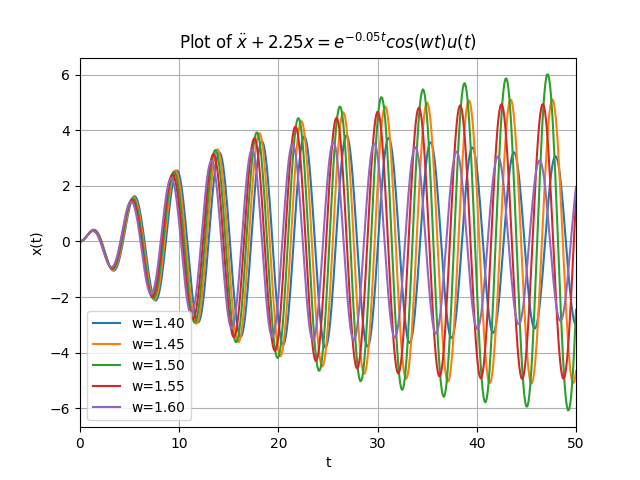
\includegraphics[scale=0.5]{figure_2.png} 
                \caption{Contour Plot of $\epsilon_{ij}$}
                \label{fig:figure_2}
            \end{figure}

            We can see that there is a minimum and  it is located approximately near the orignal function coefficients.\\

            Using the 'lstsq' function in scipy package, we solve for:
            \begin{equation}
            M.p = D \label{eq5}
            \end{equation}
            where
            \begin{equation}
            M=\left[\begin{matrix}
            J_2(t_1)&t_1\\
            ...&...\\
            J_2(t_m)&t_m
            \end{matrix}\right]\text{, }p=\left[\begin{matrix}
            A_{fit}\\B_{fit}
            \end{matrix}\right]\ \text{and }D=\left[\begin{matrix}f(t_1)\\...\\f(t_m)\end{matrix}\right]
            \end{equation}\\

            Thus, we solve for $p$ and then find the mean square error of the values of $A_{fit}$ and $B_{fit}$ found using 'lstsq' and the original values $(1.05,\ -0.105)$.

        \subsection{Finding out the variation of $\epsilon$ with $\sigma_n$}
            We solve \eqref{eq5} for different values of $\sigma_n$, by changing matrix D to different columns of 'fitting.dat'. We see that the variation of the MS error of values $A_{fit}$ and $B_{fit}$ is as follows:
            \begin{figure}[H]
                \centering
                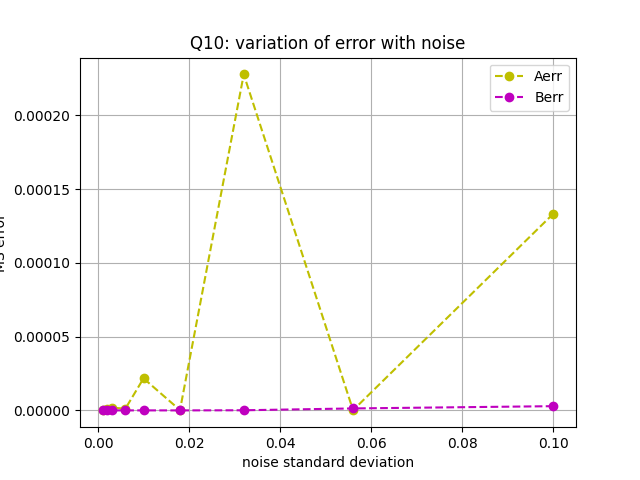
\includegraphics[scale=0.5]{figure_3.png} 
                \caption{MS Error vs Standard Deviation}
                \label{fig:figure_3}
            \end{figure}

            Except for one anomalous point near 0.03, it is approximately linear. 
            To see that more clearly, we do loglog plot below:
            \begin{figure}[H]
                \centering
                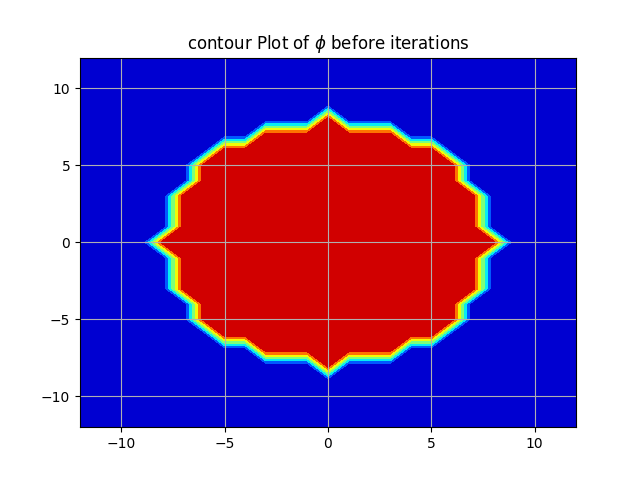
\includegraphics[scale=0.5]{figure_4.png} 
                \caption{Error vs Standard Deviation loglog Plot}
                \label{fig:figure_4}
            \end{figure}

    \section{CONCLUSION}
     we can conclude that the logarithm of the standard deviation of the noise linearly affects the logarithm of the error in the calcuation of the least error fit for a given set of data.
\end{document}
